\chapter{Routing Interior} \label{sec:ext_routing}

\section{Tipologia de rede e interfaces}

Nesta secção será abordada a implementação do protocolo de \textit{routing} exterior BGP.

O primeiro passo é definir qual é a tipologia de rede, i.e., como vão serão definidas as ligações entre os diferentes AS.
Tendo cada router de bancada um número limite de interfaces, e estando já as ligações com fios pre-configuradas, a tipologia de rede é definida da seguinte forma:

\begin{figure}[H]
    \centering
    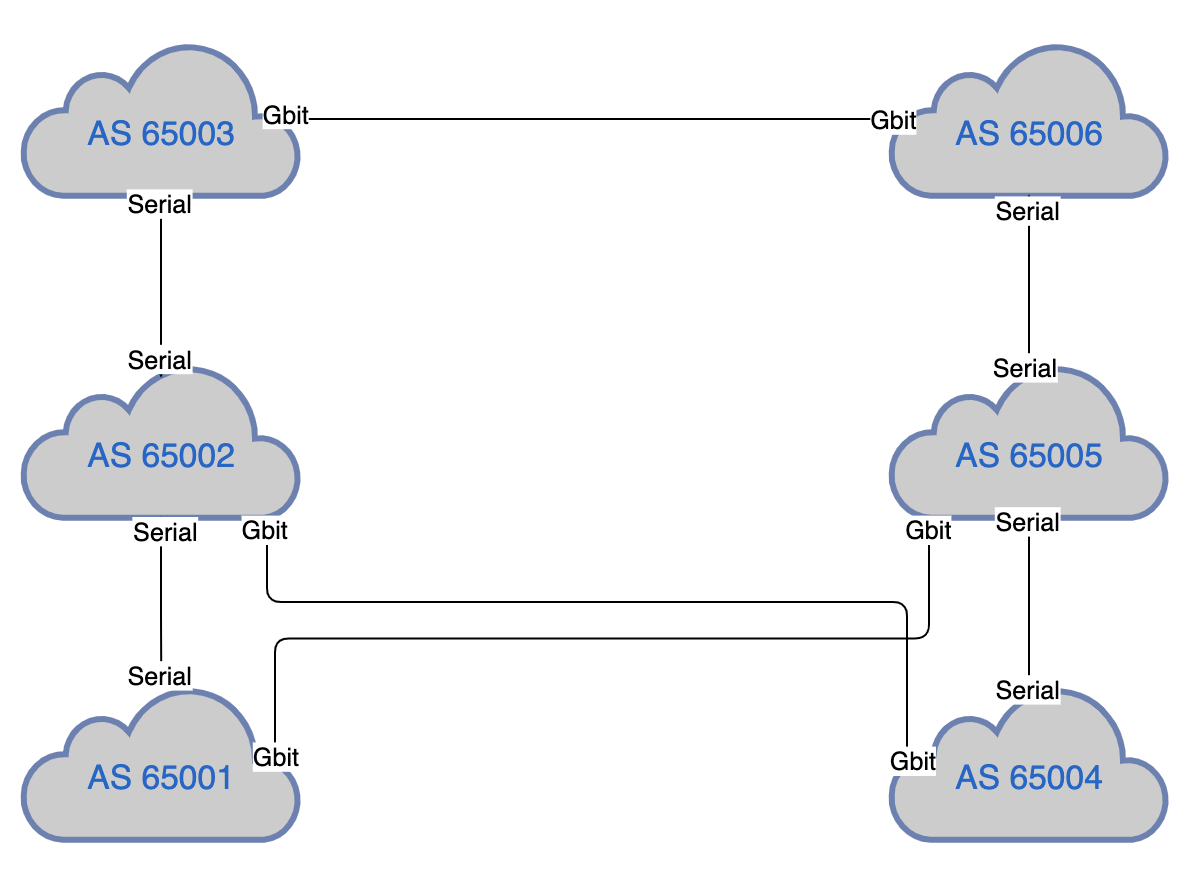
\includegraphics[width=.8\linewidth]{figs/ext_routing/bgp_tipo.png}
    \caption{Tipologia de rede com os diferentes AS e as respetivas ligações}
    \label{fig:bgp_tipo}
\end{figure}

As ligações \textit{Serial} são feitas sempre com as bancadas adjacentes.
Isto deve-se ao facto dos cabos para esta interface serem mais curtos e desse modo não conseguem se ligar aos restantes routers.

As ligações \textit{GigabitEthernet} tem como objetivo a ligação entre as duas filas de bancadas.
Já existem disponíveis ligações físicas entre todas as bancadas, onde podemos estabelecer uma ligação a todas as bancadas.
No entanto, cada router apenas tem disponível uma interface GigabitEthernet, logo apenas pode fazer uma ligação.

A AS que foi configurada foi a AS-65001.
Esta interface é composta por 4 routers, sendo que router de bancada é o \textbf{ABR} (\textit{Area Border Router}).

Como indicado no esquemático, a AS-65001 está diretamente ligada à:
\begin{itemize}
    \item AS-65002 : Rede 192.168.1.48/30 por Serial
    \item AS-65005 : Rede 192.168.1.60/30 Por GigabitEthernet
\end{itemize}

Estas duas AS são então as AS vizinhas, informação importante na configuração do processo BGP.

A configuração das duas interfaces foi feita do seguinte modo:

\begin{figure}[H]
    \centering
    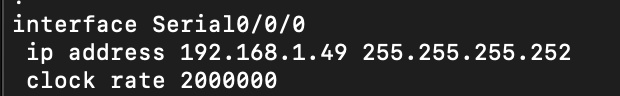
\includegraphics[width=.8\linewidth]{figs/ext_routing/serial.png}
    \caption{Atribuição do IP correspondente à interface Serial0/0/1}
    \label{fig:serial}
\end{figure}

\begin{figure}[H]
    \centering
    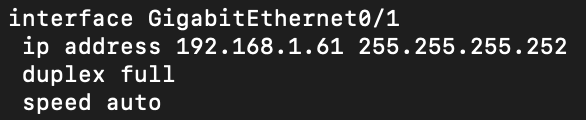
\includegraphics[width=.8\linewidth]{figs/ext_routing/giga.png}
    \caption{Atribuição do IP correspondente à interface GigabitEthernet0/1}
    \label{fig:giga}
\end{figure}


As interfaces vizinhas estão configuradas do seguinte modo:
\begin{itemize}
    \item AS-65002: Serial - Ip:192.168.1.50
    \item AS-65005: GigabitEthernet - Ip:192.168.1.62
\end{itemize}

A configuração do processo BGP no router foi a seguinte \cite{cisco_bgp}:

\begin{figure}[H]
    \centering
    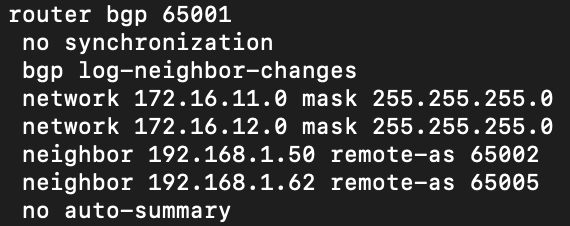
\includegraphics[width=.8\linewidth]{figs/ext_routing/bgp_router.png}
    \caption{Configuração do processo BGP 65001 no router de bancada}
    \label{fig:bgp_router}
\end{figure}

Nesta configuração são especificados:
\begin{itemize}
    \item Neighbors, neste caso o AS-65002 e AS-65005 com os respetivos IPs.
    \item Networks, que foram definidas no routing interno.
    \item \verb|no synchronization|, de forma a impedir a utilização do IBGP no routing interno
    \item \verb|bgp log-neighbor-changes|, para atualizar o status das AS vizinhas.
    \item \verb|no auto-summary| é aplicado por predefinição e não tem relevância neste contexto
\end{itemize}

\section{Teste de Routing do BGP}

\begin{figure}[H]
    \centering
    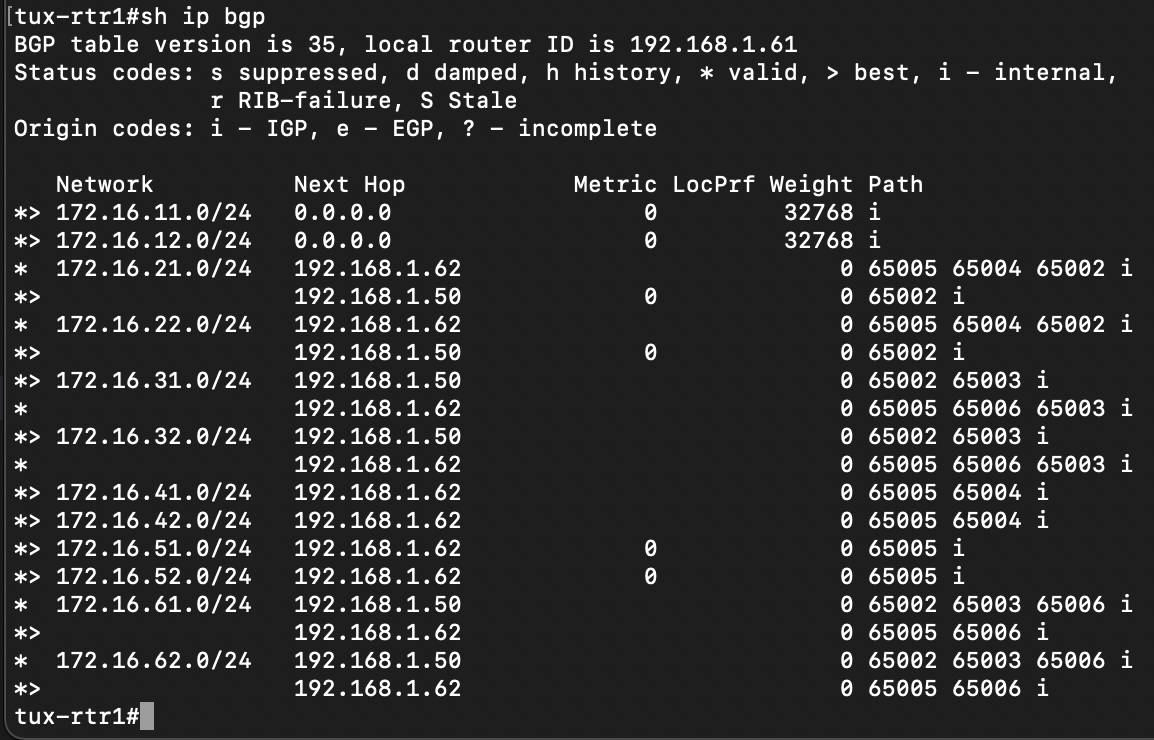
\includegraphics[width=.8\linewidth]{figs/ext_routing/bgp_table.png}
    \caption{Routing Table BGP}
    \label{fig:bgp_table}
\end{figure}

O BGP apresenta dois caminhos alternativos para cada AS, oferecendo prioridade ao caminho mais curto, i.e, que requer passar por menos AS.
No caso de dois caminhos terem o mesmo comprimento, o BGP dá prioridade ao caminho que tem como \textit{next Hop} o AS mais pequeno.
Por exemplo, na figura \ref{fig:bgp_tipo}, o AS65001 pode aceder ao AS65004 através quer do AS65002, quer do AS65005. 
Por predefinição vai escolher o AS65002.

No momento em que foi tirado o \textit{print} com a configuração, o AS65002 não tinha ligação ao AS65004.
Desse modo, apenas é fornecida uma rota possível para o AS6004 e AS6005, que corresponde à ligação direta entre o nosso AS65001 e AS6006.
Se essa ligação estivesse ativa, as rotas para o AS6006 seriam:
\begin{itemize}
    \item AS6001-AS6002-AS6004 (escolhida por ter um AS \textit{identifier} mais pequeno)
    \item AS6001-AS6605-AS6005
\end{itemize}

Para confirmar a escolha dos caminhos, são feitos \verb|traceroute|s para todas as redes:

\begin{figure}[H]
    \centering
    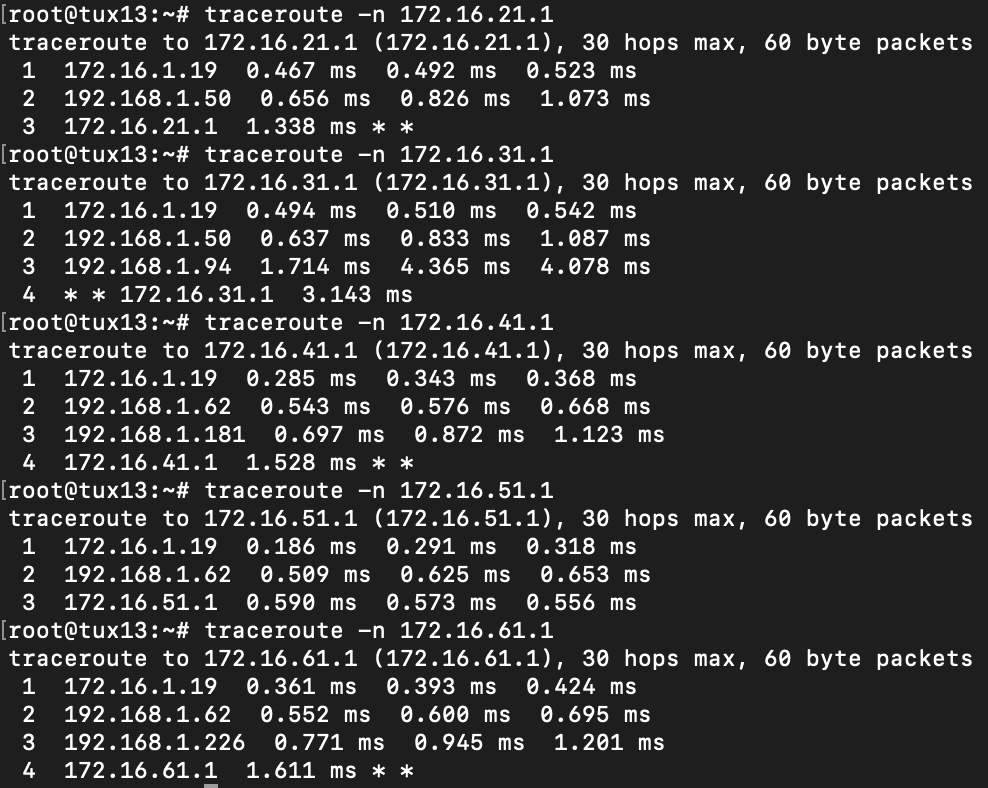
\includegraphics[width=.8\linewidth]{figs/ext_routing/traceroute_og.png}
    \caption{Traceroute para todas as redes do Tux13}
    \label{fig:traceroute_og}
\end{figure}

Como se pode observar, um acesso a um \textit{neighbor}, como o AS65002 é direto.
O primeiro IP é o acesso ao ABR, neste caso o 172.16.1.19 na AS65001.
O segundo é o IP do ABR no AS65002, na interface que liga diretamente ao AS65001, 172.16.1.50.
O terceiro é o próprio IP da rede de destino.

No caso de um acesso a um AS que não seja vizinho, como é o caso do AS65003,
temos que passar primeiro pelo AS65002 e só depois podemos ligar ao AS65003.

Todas estes caminhos são os indicados como preferenciais pelo BGP na figura \ref{fig:bgp_table}.

\pagebreak

\section{Configuração para teste - \textit{Highest AS}}

O último teste consiste em dar prioridade a rotas pelo AS com o valor mais elevado.
Como indicado anteriormente, o BGP faz precisamente o contrário por predefinição.

Relembrando o exemplo do acesso pelo AS65001 ao AS65004, queremos que seja feito pelo AS65005, e não pelo AS65004.
No entanto, no momento da elaboração deste relatório, o AS65004 não tinha conectividade ao AS65004, pelo que este cenário não é possível demonstrar.
\textbf{Nesta tipologia, não existe mais nenhum cenário para o AS6001 que esta regra possa ser testada.}

Consideramos então outro cenário que permite testar a metodologia: acesso ao AS65003.
As duas rotas possíveis são:
\begin{itemize}
    \item AS65001 -> AS65002 -> AS65003
    \item AS65001 -> AS65005 -> AS65006 -> AS65003
\end{itemize}

Como se pode observar, o segundo caminho tem mais \textit{hops}, pelo que não vai ser o escolhido pelo BGP.

\begin{figure}[H]
    \centering
    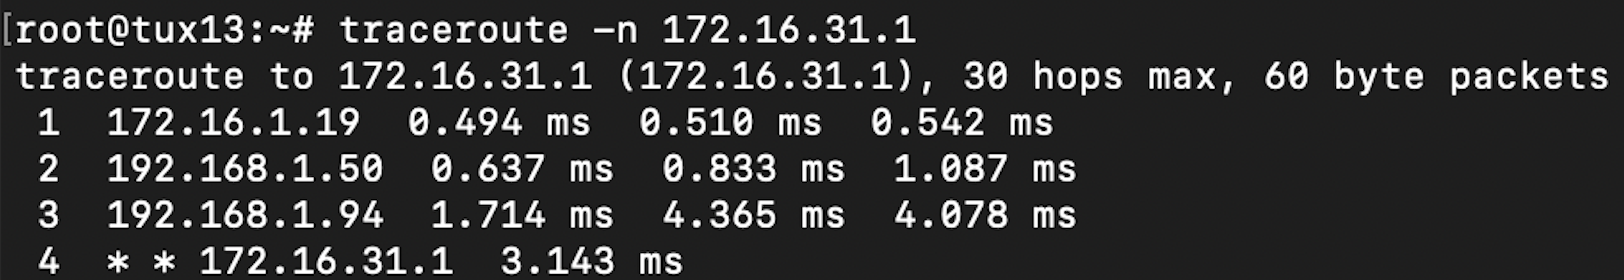
\includegraphics[width=.8\linewidth]{figs/ext_routing/traceroute_as3.png}
    \caption{Rota para o AS65003}
    \label{fig:traceroute_as3}
\end{figure}

Para se forçar este caminho, temos que aplicar uma penalização ao AS65002.

Isto é obtido com a seguinte configuração \cite{cisco_route_map}:

\begin{figure}[H]
    \centering
    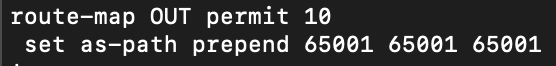
\includegraphics[width=.8\linewidth]{figs/ext_routing/route_map.png}
    \caption{Route-map OUT}
    \label{fig:route_map}
\end{figure}


Através desta configuração, estamos a adicionar 3 \textit{extra hops}, de forma a aumentar o custo do rota pelo AS65002.
O comando \verb|neighbor 192.168.1.50 route-map OUT in| adiciona estes \textit{hops} para tráfego interno, i.e., que está a sair do AS65001 para o AS65002.
Deste modo, o caminho do AS65002 para o AS65001 não tem nenhum \textit{hop} extra.
Para tal, era preciso adicionar o comando paralelo \verb|neighbor 192.168.1.50 route-map OUT out|.
Este comando adiciona \textit{extra hops} para o tráfego externo, i.e, o nosso AS não considera esse \textit{extra hops} mas os restantes consideram.

\begin{figure}[H]
    \centering
    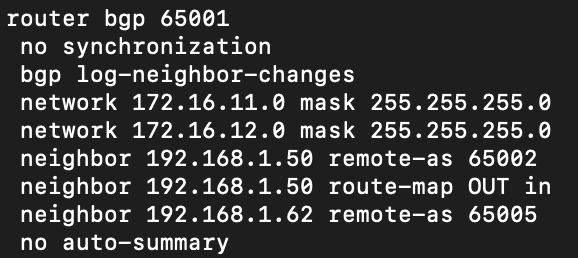
\includegraphics[width=.8\linewidth]{figs/ext_routing/bgp_router_2.png}
    \caption{Associar o route-map OUT ao AS65002}
    \label{fig:bgp_router_2}
\end{figure}

\begin{figure}[H]
    \centering
    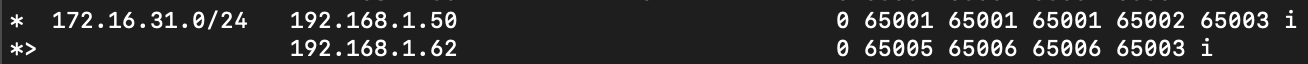
\includegraphics[width=.8\linewidth]{figs/ext_routing/route_as3_2.png}
    \caption{Novas rotas para o AS65003}
    \label{fig:route_as3_2}
\end{figure}

O AS65006 adicionou também um \textit{hop} extra para acesso feitos do AS65003.
No entanto, o custo continua a ser menor, sendo que a nova rota preferencial é pelo AS65005.

O \verb|traceroute| confirma este cenário:

\begin{figure}[H]
    \centering
    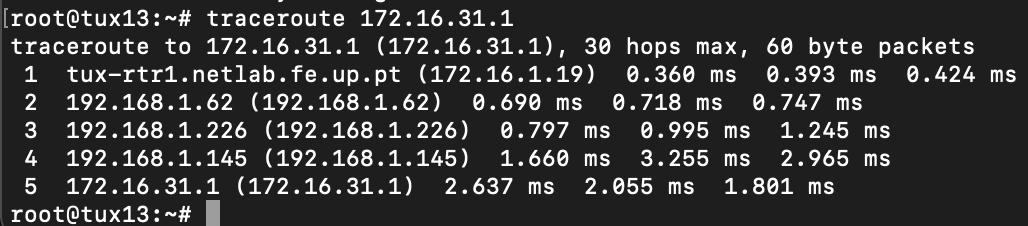
\includegraphics[width=.8\linewidth]{figs/ext_routing/traceroute_as3_2.png}
    \caption{Novo traceroute para o AS65005}
    \label{fig:traceroute_as3_2}
\end{figure}

Como se pode observar, o caminho escolhido é agora pelo AS65005 (172.168.1.62).


Nota: No final do trabalho, foi possível tirar um \textit{print} que já fornece duas rotas para cada AS.
No entanto, os restantes grupos já tinham configurado \textit{prepends}, pelo que o sistema já não está equilibrado.
No entanto, ainda é possível observar os caminhos.

\begin{figure}[H]
    \centering
    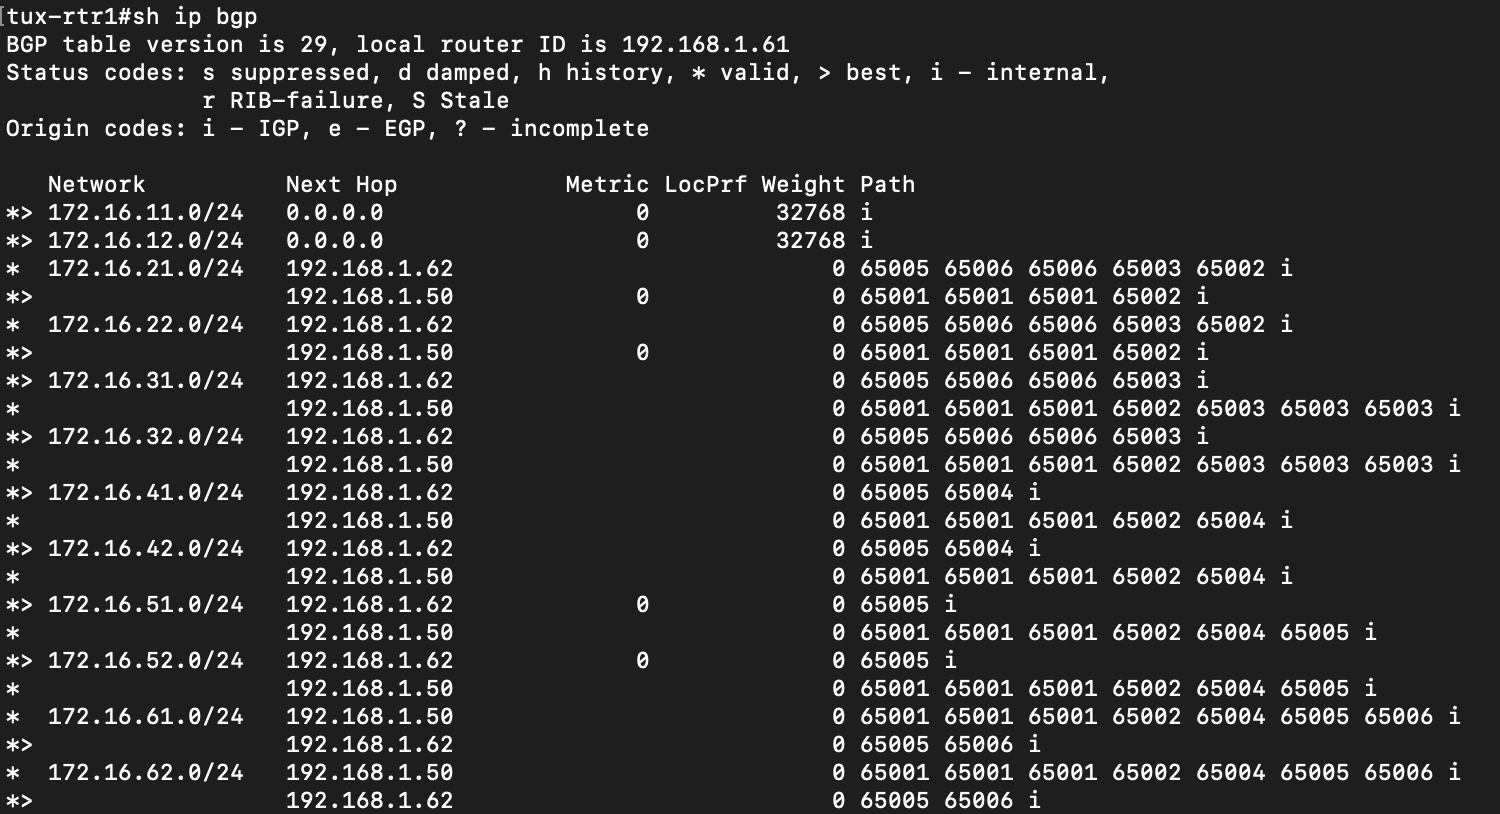
\includegraphics[width=.8\linewidth]{figs/ext_routing/route_bgp_extra.png}
    \caption{Rotas para os diferentes AS}
    \label{fig:route_bgp_extra}
\end{figure}





